\documentclass[runningheads,a4paper]{llncs}

\usepackage[utf8]{inputenc}
\usepackage[T1]{fontenc}
\usepackage[brazilian]{babel}
\usepackage{hyphenat}
\hyphenation{pro-ble-ma}

\usepackage{amssymb}
\usepackage{amsmath}
\usepackage{array}

\usepackage{multirow}
\newcommand{\breakcell}[2][c]{%
	\begin{tabular}[#1]{@{}c@{}}#2\end{tabular}}

%better font, similar to the default springer font
%cfr-lm is preferred over lmodern. Reasoning at http://tex.stackexchange.com/a/247543/9075
\usepackage[%
rm={oldstyle=false,proportional=true},%
sf={oldstyle=false,proportional=true},%
tt={oldstyle=false,proportional=true,variable=true},%
qt=false%
]{cfr-lm}
%
%if more space is needed, exchange cfr-lm by mathptmx
%\usepackage{mathptmx}

\usepackage{graphicx}
\graphicspath{ {images/} }

%extended enumerate, such as \begin{compactenum}
\usepackage{paralist}

%put figures inside a text
%\usepackage{picins}
%use
%\piccaptioninside
%\piccaption{...}
%\parpic[r]{\includegraphics ...}
%Text...

%Sorts the citations in the brackets
%\usepackage{cite}

%for easy quotations: \enquote{text}
\usepackage{csquotes}

%enable margin kerning
\usepackage{microtype}

%for demonstration purposes only
\usepackage[math]{blindtext}

%tweak \url{...}
\usepackage{url}
%nicer // - solution by http://tex.stackexchange.com/a/98470/9075
\makeatletter
\def\Url@twoslashes{\mathchar`\/\@ifnextchar/{\kern-.2em}{}}
\g@addto@macro\UrlSpecials{\do\/{\Url@twoslashes}}
\makeatother
\urlstyle{same}
%improve wrapping of URLs - hint by http://tex.stackexchange.com/a/10419/9075
\makeatletter
\g@addto@macro{\UrlBreaks}{\UrlOrds}
\makeatother

%diagonal lines in a table - http://tex.stackexchange.com/questions/17745/diagonal-lines-in-table-cell
%slashbox is not available in texlive (due to licensing) and also gives bad results. This, we use diagbox
%\usepackage{diagbox}

%required for pdfcomment later
\usepackage{xcolor}

% new packages BEFORE hyperref
% See also http://tex.stackexchange.com/questions/1863/which-packages-should-be-loaded-after-hyperref-instead-of-before

%enable hyperref without colors and without bookmarks
\usepackage[
%pdfauthor={},
%pdfsubject={},
%pdftitle={},
%pdfkeywords={},
bookmarks=false,
breaklinks=true,
colorlinks=true,
linkcolor=black,
citecolor=black,
urlcolor=black,
%pdfstartpage=19,
pdfpagelayout=SinglePage,
pdfstartview=Fit
]{hyperref}
%enables correct jumping to figures when referencing
\usepackage[all]{hypcap}

%enable nice comments
\usepackage{pdfcomment}
\newcommand{\commentontext}[2]{\colorbox{yellow!60}{#1}\pdfcomment[color={0.234 0.867 0.211},hoffset=-6pt,voffset=10pt,opacity=0.5]{#2}}
\newcommand{\commentatside}[1]{\pdfcomment[color={0.045 0.278 0.643},icon=Note]{#1}}

%compatibality with TODO package
\newcommand{\todo}[1]{\commentatside{#1}}

%enable \cref{...} and \Cref{...} instead of \ref: Type of reference included in the link
\usepackage[capitalise,nameinlink]{cleveref}
%Nice formats for \cref
\crefname{section}{Sect.}{Sect.}
\Crefname{section}{Section}{Sections}
\crefname{figure}{Fig.}{Fig.}
\Crefname{figure}{Figure}{Figures}

\usepackage{xspace}
%\newcommand{\eg}{e.\,g.\xspace}
%\newcommand{\ie}{i.\,e.\xspace}
\newcommand{\eg}{e.\,g.,\ }
\newcommand{\ie}{i.\,e.,\ }

%introduce \powerset - hint by http://matheplanet.com/matheplanet/nuke/html/viewtopic.php?topic=136492&post_id=997377
\DeclareFontFamily{U}{MnSymbolC}{}
\DeclareSymbolFont{MnSyC}{U}{MnSymbolC}{m}{n}
\DeclareFontShape{U}{MnSymbolC}{m}{n}{
    <-6>  MnSymbolC5
   <6-7>  MnSymbolC6
   <7-8>  MnSymbolC7
   <8-9>  MnSymbolC8
   <9-10> MnSymbolC9
  <10-12> MnSymbolC10
  <12->   MnSymbolC12%
}{}
\DeclareMathSymbol{\powerset}{\mathord}{MnSyC}{180}

\begin{document}

%Works on MiKTeX only
%hint by http://goemonx.blogspot.de/2012/01/pdflatex-ligaturen-und-copynpaste.html
%also http://tex.stackexchange.com/questions/4397/make-ligatures-in-linux-libertine-copyable-and-searchable
%This allows a copy'n'paste of the text from the paper
\input glyphtounicode.tex
\pdfgentounicode=1

\title{Aprendizado Multirrótulo Aplicado a Predição de Ocupações para Oportunidades de Trabalho}
%If Title is too long, use \titlerunning
\titlerunning{Aprendizado Multirrótulo}

%Single insitute
\author{
	Ronie Uliana e Leandro Nunes de Castro
}
%If there are too many authors, use \authorrunning
%\authorrunning{First Author et al.}
\institute{Universidade Presbiteriana Mackenzie}

%Multiple insitutes
%Currently disabled
%
\iffalse
%Multiple institutes are typeset as follows:
\author{Firstname Lastname\inst{1} \and Firstname Lastname\inst{2} }
%If there are too many authors, use \authorrunning
%\authorrunning{First Author et al.}

\institute{
Insitute 1\\
\email{...}\and
Insitute 2\\
\email{...}
}
\fi
			
\maketitle

\begin{abstract}
Esse trabalho é um estudo de caso que apresenta os resultados da aplicação de classificação multirrótulo em um problema de recrutamento de pessoas. O trabalho tenta prever quais ocupações serão atraídas para uma oportunidade de trabalho dependendo exclusivamente do título anunciado.
\end{abstract}

\keywords{multirrótulo,classificação,\textit{ensemble},contratação,recursos humanos}

\section{Introdução} \label{sec:intro}

O título anunciado em uma oportunidade de trabalho tem grande influência no tipo de pessoa que a oportunidade atrai. Um vaga com o título \enquote{Engenheiro de Custos} atrai principalmente engenheiros civis, já uma intitulada \enquote{Engenheiro Civil Júnior} tem grandes chances de atrair pessoas que atualmente são estagiários de Engenharia Civil.

Esse trabalho usa uma base de dados de mercado para tentar prever quais ocupações são atraídas pelo título da vaga. Ela acumula informação de 16 anos de uma empresa que possui um produto para o mercado de Recrutamento e Seleção e possui pouco menos de meio milhão de oportunidades de trabalho.

Os resultados mostram que é possível prever bastante bem quais são as ocupações para essas oportunidades utilizando somente o título anunciado. A intenção é incorporar o modelo gerado nesse trabalho para ajudar os recrutadores a criarem oportunidades mais assertivas.

Além do caso em questão, é natural o uso de mais de um rótulo em outros problemas. Por exemplo, na classificação de textos, uma reportagem sobre o Oriente Médio pode ser classificada como jornalismo, política ou árabe, entre outros rótulos. Uma fotografia qualquer pode ter múltiplos elementos como um barco, o mar e montanhas ao fundo e cada um desses elementos pode ser considerado um rótulo.

O aprendizado multirrótulo é um aprendizado supervisionado e procura encontrar o \emph{conjunto} de rótulos associado a um registro. Nesse trabalho, foi adotado o termo "aprendizado" ao invés de classificação pois essa área estuda tanto o aprendizado de funções de classificação quanto de ordenação, explicados em mais detalhes na seção \ref{sec:classord} \cite{Zhang2014-be}.

As próximas seções apresentam uma visão geral e uma breve revisão das pesquisas relevantes na área de classificação multirrótulo, com maior detalhamento nas técnicas selecionadas para o trabalho. A seguir, a seção \ref{sec:formal} define formalmente os problemas de classificação e ordenação multirrótulo, nela também é apresentada a notação matemática usada no restante do trabalho. 

Logo depois, a seção \ref{sec:metricas} apresenta métricas usadas para caracterização dos problemas de aprendizado multirrótulo, ao invés de uma lista extensa ela é restrita a três das métricas mais relevantes para o problema tratado nesse trabalho. Nas seções \ref{sec:justificativa} e \ref{sec:preparacao}, é apresentada uma justificativa para a escolha do método e  um resumo dos processos empregados para limpeza e seleção dos dados.

A seção \ref{sec:aplicacao} detalha aplicação do método, enquanto a seção \ref{sec:resultados} apresenta os resultados obtidos. Finalmente a última seção \ref{sec:conclusao} faz considerações sobre o trabalho, destacando pontos de interesse e limitações dos resultados obtidos.

\section{Transformação do Problema e Adaptação do Algoritmo}

A tarefa de aprendizado multirrótulo pode ser divida em dois tipos principais, dependendo da estratégia para abordá-la \cite{Tsoumakas2009-vw}. A primeira abordagem consiste em transformá-la em um problema de \textit{classificação multiclasse}, para o qual já existe extensa literatura e estudo. A segunda abordagem \textit{adapta algoritmos} usados na classificação multiclasse para que sejam capazes de lidar com múltiplos rótulos.

Algumas das adaptações de algoritmos como [TODO listá-las aqui] fazem, na verdade, transformações do problema dentro da adaptação.

\section{Classificação e Ordenação Multirrótulo} \label{sec:classord}

A classificação consiste em encontrar um subconjunto de rótulos que esteja corretamente associado a um exemplo. Já a ordenação não cria um subconjunto a ser associado ao registro, ao invés disso, procura estabelecer uma ordem entre o todos os rótulos. Aqueles com maior confiança de pertencer ao registro são colocados antes daqueles com menor confiança.

Um ordenação multirrótulo é transformada em uma classificação se em algum ponto da ordem for estabelecido um corte e apenas os rótulos em posições melhores forem considerados. Esse \enquote{conjunto dos melhores} é o conjunto resposta para a classificação.

\section{Ordens de Correlação}

Uma das características únicas da aprendizagem multirrótulo é que, em problema reais, rótulos costumam coocorrer ou seguir uma certa relação hierárquica. Por exemplo, uma imagem que possua o rótulo "prato" estará mais frequentemente associada com os rótulos "cozinha" ou "ingredientes" do que com rótulos como "praia" ou "areia". Estratégias que se aproveitam da relação entre rótulos parecem ter melhor desempenho do que as que as ignoram \cite{Zhang2010-ee}.

É possível distinguir três tipos de estratégias quanto a correlação entre rótulos, de primeira, segunda ordem e de ordem superior.

\subsection{Correlação de Primeira Ordem.} \label{subsec:corr1ordem}

A correlação entre os rótulos não é explorada, a predição para cada rótulo é aprendida separadamente, ou seja, \emph{uma-a-uma}. O conjunto de rótulos predito para cada registro é uma união do resultado de cada aprendizado \cite{De_Carvalho2009-yp}.

As estratégias de cópia e seleção nas seções \ref{subsec:copia}, \ref{subsec:copiaponderada}, \ref{subsec:selecaominimo}, \ref{subsec:selecaomaximo} e \ref{subsec:selecaoaleatoria} mostram exemplos de transformações com correlações de primeira ordem, bom como a \textit{Relevância Binária} (seção \ref{subsec:relevanciabinaria}).

\subsection{Correlação de Segunda Ordem.} \label{subsec:corr2ordem}

A correlação é explorada no formato \emph{dois-a-dois}. Cada par de rótulos é aprendido por um classificador diferente e o conjunto final é predito através da combinação entre os pares \cite{Hullermeier2008-co}.

A estratégia de comparação entre duplas na seção \ref{subsec:comparacaoduplas} usa correlação de segunda ordem.

\subsection{Correlação de Ordem Superior.} \label{subsec:corrSordem}

Explora-se a correlação entre conjuntos maiores de rótulos \cite{Read2008-bt}, entre subconjuntos aleatórios entre si \cite{Tsoumakas2007-cw} ou com relações de hierarquia entre rótulos \cite{Cesa-Bianchi2006-fk}.

As estratégias RAkEL e \textit{Ensemble of Pruned Sets} nas seções \ref{subsec:rakel} e \ref{subsec:eps} são exemplos de correlação de ordem superior.

\section{Definição Formal do Problema} \label{sec:formal}

Chamamos de $\mathcal{X}$ o conjunto de registros e de $\mathcal{Y}$ o conjunto com todos os rótulos possíveis. O conjunto potência $2^{\mathcal{Y}}$ é o conjunto com todos os subconjuntos possíveis de $\mathcal{Y}$.

Define-se então, formalmente, o problema de classificação multirrótulo como encontrar $h : \mathcal{X} \to 2^\mathcal{Y}$ , ou seja, encontrar a função que, dado um registro, encontra o conjunto de rótulos que mais provavelmente caracterizam o registro.

Usando a mesma notação, define-se a tarefa de ordenação multirrótulo como encontrar $f : \mathcal{X} \to \mathbb{R}$ (ou $f : \mathcal{X} \to \mathbb{Z}$) a função que, dado um rótulo e um registro, retorna um valor que representa a confiança de que aquele rótulo seja correto para o registro.

Para conveniência, as tabelas \ref{tab:matematica-registros}, \ref{tab:matematica-rotulos} e \ref{tab:matematica-funcoes} contêm as definições matemáticas usadas no restante do trabalho.

\begin{table}
	\centering
	\begin{tabular}{| >{\centering}p{4cm} | m{8cm} |}
		\hline
		\multicolumn{2}{|c|}{\textit{Registros ou vetores de atributos}} \\
		\hline
		$\mathcal{X} = \mathbb{R}^d \vee \mathcal{X} = \mathbb{Z}^d$ & $\mathcal{X}$ é o conjunto que abrange todos os registros, também pode ser entendido como o conjunto de todos os vetores de atributos (cada vetor é um registro). \\
		\hline
		$d \in \mathbb{N}_{>0}$ & $d$ é o número de atributos nos registros, também pode ser compreendido como o número de dimensões nos vetores de atributos. \\
		\hline
		$\mathcal{X} = \{\vec{x_1}, \vec{x_2}, \dots, \vec{x_n}\}$ & Mesma definição de $\mathcal{X}$ acima, mas enumerando seus elementos. \\
		\hline
		$\vec{x_i} \in \mathcal{X}$ & $\vec{x_i}$ representa um registro ou um vetor de atributos. \\
		\hline
		$\vec{x_i} = \{x_{i1}, x_{i2}, \dots, x_{id}\}$ & $\vec{x_i}$ representa um único registro do conjunto ou um vetor com $d$ atributos. No caso, $x_{ij}$ representa o valor de um único atributo. \\
		\hline
		$n = |\mathcal{X}|$ & $n$ é o número total de registros no problema. \\
		\hline
	\end{tabular}
	\caption{Notação usada para registros}
	\label{tab:matematica-registros}
\end{table}

\begin{table}
	\centering
	\begin{tabular}{| >{\centering}p{4cm} | m{8cm} |}
		\hline	
		\multicolumn{2}{|c|}{\textit{Rótulos e conjuntos de rótulos}} \\
		\hline
		$\mathcal{Y} = \{y_1, y_2, \dots, y_q\}$ & $\mathcal{Y}$ é o conjunto com todos os rótulos possíveis para o problema. \\
		\hline
		$y_i \in \mathcal{Y}$ & $y_i$ representa um único rótulo. \\
		\hline
		$q = |\mathcal{Y}|$ & $q$ é o número de rótulos possíveis no problema. \\
		\hline
		$2^\mathcal{Y}$ & $2^\mathcal{Y}$ representa todos os subconjuntos possíveis de rótulos no problema (conjunto potência). \\
		\hline
		$L = {Y_1, Y_2, \dots, Y_n}$ & $L$ é o subconjunto de $2^\mathcal{Y}$ que contém apenas os conjuntos de rótulos encontrados no problema. \\
		\hline
		$Y_i \subseteq \mathcal{Y} \wedge Y_i \in L$ & $Y_i$ é o conjunto de rótulos associado ao registro $x_i$. \\
		\hline
	\end{tabular}
	\caption{Notação usada para os rótulos}
	\label{tab:matematica-rotulos}
\end{table}

\begin{table}
	\centering
	\begin{tabular}{| >{\centering}p{6cm} | m{6cm} |}
		\hline	
		\multicolumn{2}{|c|}{\textit{Conjuntos de treino e teste}} \\
		\hline
		$\mathcal{D} = \{(\vec{x_1}, Y_1), (\vec{x_2}, Y_2), \dots, (\vec{x_1}, Y_n)\}$ & $\mathcal{D}$ é o conjunto com todos os registros do problema com seus respectivos conjuntos de rótulos. \\
		\hline
		$\mathcal{T} = \{(\vec{x_i}, trans(Y_i)) | cort(Y_i) \}$ & $\mathcal{T}$ é o conjunto usado para treinamento, dependendo da estratégia ou do algoritmo usado ele é menor que o conjunto total ou então possui seus rótulos transformados. \\
		\hline
		$trans : 2^\mathcal{Y} \to \mathcal{Y'}$ & $trans$ é uma função que transforma um conjunto de rótulos em um rótulo único. $\mathcal{Y'}$ é o conjunto de rótulos transformados. \\
		\hline
		$cort : 2^\mathcal{Y} \to \{Verdadeiro, Falso\}$ & $cort$ é uma função que retorna Verdadeiro se um conjunto de rótulo deve integrar o conjunto de treinamento e Falso caso contrário. \\
		\hline
	\end{tabular}
	\caption{Conjuntos de treino e teste}
	\label{tab:matematica-dominio}
\end{table}

\begin{table}
	\centering
	\begin{tabular}{| >{\centering}p{4cm} | m{8cm} |}
		\hline
		\multicolumn{2}{|c|}{\textit{Funções}} \\
		\hline
		$h : \mathcal{X} \to 2^\mathcal{Y}$ & $h$ é a função que mapeia os registros em subconjuntos de rótulos. Encontrar $h$ é a tarefa principal da \textbf{classificação multirrótulo}. \\
		\hline
		$f : \mathcal{X} \times \mathcal{Y} \to \mathbb{R}$ & $f$ é a função que mapeia os registros e rótulos em um número que representa a confiança que aquele é um rótulo apropriado para o registro. Encontrar $f$ é a tarefa principal da \textbf{ordenação multirrótulo}. \\
		\hline
	\end{tabular}
	\caption{Funções de classificação e ordenação}
	\label{tab:matematica-funcoes}
\end{table}	

\section{Métricas para Caracterização do Problema} \label{sec:metricas}

As três métricas a seguir \cite{Zhang2014-be} são úteis para se entender resumidamente as características de um problema multirrótulo. Também é possível usá-las para se compreender o comportamento das estratégias e algoritmos propostos, por exemplo, alguns deles sofrem quando existe uma diversidade muito grande nos conjuntos de rótulos, provocando complicações de desbalanceamento quando são transformam o problema em multiclasse. 

A \textit{cardinalidade} de rótulos é a quantidade média de deles por registro $card(D) = \frac{1}{n} \sum_{i = 1}^{n} |Y_i|$.

A \textit{densidade} de rótulos é a proporção entre a cardinalidade e a quantidade de registros$dens(D) = \frac{1}{q} card(D)$.

A \textit{diversidade} mede a quantidade de conjuntos distintos de rótulos no problema $diver(D) = |L|$. Uma diversidade pequena em um conjunto grande de rótulos indica que alguns coocorrem com muita frequência, implicando um possível relacionamento entre eles.

\section{Transformação do Problema}\label{sec:transprob}

Existem várias estratégias que transformam um problema multirrótulo em um problema mais simples ou em um conjunto de problemas que já possuem soluções. Quase todas as estratégias abaixo transformam o problema de multirrótulo para multiclasse. Alguns deles como o \textit{RAkEL} \cite{Tsoumakas2007-wm} e o \textit{Ensemble of Pruned Sets} \cite{Read2008-bt} possuem métodos para incorporar novamente a variedade de rótulos nas respostas dos classificadores.

O conjunto de registros na tabela \ref{tab:exbase} é usado para ilustrar as diversas estratégias de transformação.

Todas as transformações por cópia e seleção ignoram a relação entre os rótulos, por isso são métodos de \textit{correlação de primeira ordem} (seção \ref{subsec:corr1ordem}).

\begin{table}
	\centering
	\begin{tabular}{| c | c |}
		\hline
		\textbf{Registro} & \textbf{Rótulos} \\
		\hline
		$\vec{x_1}$ & $y_1$ \\
		\hline
		$\vec{x_2}$ & $y_2, y_3$ \\
		\hline
		$\vec{x_3}$ & $y_3$ \\
		\hline
		$\vec{x_4}$ & $y_3, y_4, y_5$ \\
		\hline
		$\vec{x_5}$ & $y_3, y_5$ \\
		\hline
	\end{tabular}
	\caption{Exemplos de registros}
	\label{tab:exbase}
\end{table}

\subsection{Transformação por Cópia} \label{subsec:copia}

A transformação mais simples consiste em copiar os registros uma vez para cada rótulo. Usando a tabela de registros \ref{tab:exbase}, a transformação por cópia resulta na tabela \ref{tab:excopia}.

\begin{table}
\parbox{.45\linewidth}{
	\centering
	\begin{tabular}{| c | c |}
		\hline
		\textbf{Registro} & \textbf{Rótulo} \\
		\hline
		$\vec{x_1}$ & $y_1$ \\
		\hline
		$\vec{x_2}$ & $y_2$ \\
		\hline
		$\vec{x_2}$ & $y_3$ \\
		\hline
		$\vec{x_3}$ & $y_3$ \\
		\hline
		$\vec{x_4}$ & $y_3$ \\
		\hline
		$\vec{x_4}$ & $y_4$ \\
		\hline
		$\vec{x_4}$ & $y_5$ \\
		\hline
		$\vec{x_5}$ & $y_3$ \\
		\hline
		$\vec{x_5}$ & $y_5$ \\
		\hline
	\end{tabular}
	\caption{Transformação por cópia}
	\label{tab:excopia}
}
\parbox{.45\linewidth}{
	\centering
	\begin{tabular}{| c | c | c |}
		\hline
		\textbf{Registro} & \textbf{Rótulo} & \textbf{Peso ($w$)} \\
		\hline
		$\vec{x_1}$ & $y_1$ & $1$ \\
		\hline
		$\vec{x_2}$ & $y_2$ & $\frac{1}{2}$ \\
		\hline
		$\vec{x_2}$ & $y_3$ & $\frac{1}{2}$ \\
		\hline
		$\vec{x_3}$ & $y_3$ & $1$ \\
		\hline
		$\vec{x_4}$ & $y_3$ & $\frac{1}{3}$ \\
		\hline
		$\vec{x_4}$ & $y_4$ & $\frac{1}{3}$ \\
		\hline
		$\vec{x_4}$ & $y_5$ & $\frac{1}{3}$ \\
		\hline
		$\vec{x_5}$ & $y_3$ & $\frac{1}{2}$ \\
		\hline
		$\vec{x_5}$ & $y_5$ & $\frac{1}{2}$ \\
		\hline
	\end{tabular}
	\caption{Cópia ponderada}
	\label{tab:excopiapond}
}
\end{table}

É possível observar que o número de registros cresce de acordo com o número de rótulos. Formalmente, descreve-se que cada registro $(x_i,Y_i)$ é multiplicado $|Y_i|$ vezes, substituindo $Y_i$ por $y_j \in Y_i$ em cada cópia, resultando em $(x_{i}, y_j)$. O número de registros passa de $|\mathcal{X}|$ para $\sum_{i=1}^{n}|Y_i|$.

Essa transformação pode ser usada com um \textit{ensemble} de classificadores para gerar o conjunto final de rótulos \cite{Joachims1998-zz} \cite{Yang1999-ah}.

\subsection{Transformação por Cópia Ponderada} \label{subsec:copiaponderada}

Da mesma forma que a cópia do registros, mas cada rótulo recebe um valor associado que representa sua participação no registro $w = \frac{1}{|Y_i|}$. A tabela \ref{tab:excopiapond} mostra o resultado da aplicação desse método.

\subsection{Transformação pela Seleção do Mínimo} \label{subsec:selecaominimo}

Nessa transformação, o rótulo menos frequente no conjunto $\mathcal{Y}$ é selecionado para descrever cada registro.

Dada a função $freq : \mathcal{Y} \to \mathbb{N}_0$ como a função que retorna o número de ocorrências de um rótulo em todo o conjunto de rótulos $L$, cada registro $(x_i, Y_i)$ é transformado em:

$$(x_i, \min_{\forall q \in Y_i} freq(q))$$

A tabela \ref{tab:exselmin} mostra o resultado da seleção do mínimo.

\begin{table}
\parbox{.45\linewidth} {
	\centering
	\begin{tabular}{| c | c |}
		\hline
		\textbf{Registro} & \textbf{Rótulos} \\
		\hline
		$\vec{x_1}$ & $y_1$ \\
		\hline
		$\vec{x_2}$ & $y_2$ \\
		\hline
		$\vec{x_3}$ & $y_3$ \\
		\hline
		$\vec{x_4}$ & $y_4$ \\
		\hline
		$\vec{x_5}$ & $y_5$ \\
		\hline
	\end{tabular}
	\caption{Seleção do mínimo}
	\label{tab:exselmin}
}
\parbox{.45\linewidth}{
	\centering
	\begin{tabular}{| c | c |}
		\hline
		\textbf{Registro} & \textbf{Rótulos} \\
		\hline
		$\vec{x_1}$ & $y_1$ \\
		\hline
		$\vec{x_2}$ & $y_2$ \\
		\hline
		$\vec{x_3}$ & $y_3$ \\
		\hline
		$\vec{x_4}$ & $y_4$ \\
		\hline
		$\vec{x_5}$ & $y_5$ \\
		\hline
	\end{tabular}
	\caption{Seleção do máximo}
	\label{tab:exselmax}
}
\end{table}

\subsection{Transformação pela Seleção do Máximo} \label{subsec:selecaomaximo}

Na seleção do máximo, cada o rótulo selecionado para representar cada registro é o que ocorre com mais frequência no conjunto $\mathcal{Y}$.

Similar à seleção do mínimo, cada registro $(x_i, Y_i)$ é transformado em:

$$(x_i, \max_{\forall q \in Y_i} freq(q))$$

A tabela \ref{tab:exselmax} mostra um exemplo dessa transformação.

\subsection{Transformação por Seleção Aleatória} \label{subsec:selecaoaleatoria}

A seleção aleatória simplesmente seleciona um único rótulo aleatoriamente do conjunto para representar o registro.

Dada a função $rand : 2^\mathcal{Y} \to \mathcal{Y}$ que retorna um rótulo qualquer de um conjunto de rótulos recebidos, cada registro é transformado $(x_i, Y_i)$ em $(x_i, rand(Y_i))$.

\begin{table}
\parbox{.45\linewidth}{
	\centering
	\begin{tabular}{| c | c |}
		\hline
		\textbf{Registro} & \textbf{Rótulos} \\
		\hline
		$\vec{x_1}$ & $y_1$ \\
		\hline
		$\vec{x_2}$ & $y_3$ \\
		\hline
		$\vec{x_3}$ & $y_3$ \\
		\hline
		$\vec{x_4}$ & $y_5$ \\
		\hline
		$\vec{x_5}$ & $y_3$ \\
		\hline
	\end{tabular}
	\caption{Seleção aleatória}
	\label{tab:exrand}
}
\parbox{.45\linewidth}{
	\centering
	\begin{tabular}{| c | c |}
		\hline
		\textbf{Registro} & \textbf{Rótulos} \\
		\hline
		$\vec{x_1}$ & $y_1$ \\
		\hline
		$\vec{x_3}$ & $y_3$ \\
		\hline
	\end{tabular}
	\caption{Ignorando multirrótulos}
	\label{tab:exignora}
}
\end{table}

\subsection{Transformação por Ignorar Multirrótulo} \label{subsec:ignorarmultirrotulo}

Essa transformação simples reduz o número de registros de treino ignorando todos aqueles que possuem mais de um único rótulo.

O conjunto resultante é formado por $\{ (x_i, Y_i) \mid |Y_i| = 1 \}$


Se a cardinalidade for próxima de 1 essa técnica pode ser apropriada, embora o resultado da transformação fique muito próximo da \textit{transformação por cópia}.

Com cardinalidades mais altas, esse método pode remover uma quantidade significativa de registros.

\subsection{Relevância Binária} \label{subsec:relevanciabinaria}

As estratégias de transformação usam, em grande parte, um \textit{ensemble} de classificadores binários \cite{Zhang2014-be}. Variações da estratégia descrita aqui são base para várias outras mais elaboradas. Para problemas multiclasse, essa estratégia é conhecida como \textit{one-vs-all} ou \textit{one-vs-rest}.

Na sua forma mais simples, cada classificador é treinado para identificar uma única ocorrência do rótulo. No conjunto de treinamento, se o rótulo existe no registro, recebe o valor 1, caso contrário, recebe -1 (ou 0, dependendo da estratégia).

\begin{align*}
\mathcal{T}_k& = \{ (\vec{x}, trans(Y_i, y_k)) | 1 \leq i \leq n \} \\
\text{onde } trans(Y_i, y_k) &= \begin{cases}
				 				  +1, \text{se $y_k \in Y_i$}\\
								  -1, \text{caso contrário.}
			  				    \end{cases}
\end{align*}

O conjunto resposta é formado por todos os rótulos em que seus classificadores responderam positivamente. Como nem o treinamento, nem a votação, levam em conta a relação entre rótulos, ela é uma estratégia com \textit{correlação de primeira ordem} (seção \ref{subsec:corr1ordem}).

\subsection{Transformação por Conjunto Potência (\textit{Label Powerset})} \label{subsec:conjuntopotencia}

Na sua versão mais simples, essa estratégia transforma cada conjunto possível de rótulos em um único rótulo novo. Por exemplo, o conjunto de rótulos $\mathcal{Y} = \{a, b, c\}$ se transforma nos rótulos $\mathcal{Y'} = \{a, b, c, ab, bc, ac, abc\}$. O número de classes geradas dessa maneira é $2^q$.

\begin{table}
	\centering
	\begin{tabular}{| c | c |}
		\hline
		\textbf{Registro} & \textbf{Rótulos} \\
		\hline
		$\vec{x_1}$ & $y_1$ \\
		\hline
		$\vec{x_2}$ & $y_{2, 3}$ \\
		\hline
		$\vec{x_3}$ & $y_3$ \\
		\hline
		$\vec{x_4}$ & $y_{3, 4, 5}$ \\
		\hline
		$\vec{x_5}$ & $y_{3, 5}$ \\
		\hline
	\end{tabular}
	\caption{Conjunto potência concatena rótulos}
	\label{tab:expotencia}
\end{table}


Na prática, a quantidade de rótulos está limitada ao conjunto de registros $\min(n, 2^q)$. Se a \textit{densidade} do conjunto for baixa e a \textit{diversidade} for alta, essa estratégia acaba criando classes muito desbalanceadas, o que requer outras técnicas para o treinamento, como detecção de anomalias. Apesar disso, explora bastante bem a relação entre os rótulos \cite{Read2008-bt} pois forma \textit{correlações de segunda ordem}.

As estratégias \textit{RAkEL} \cite{Tsoumakas2007-wm} e \textit{Ensemble of Pruned Sets} \cite{Read2008-bt} descritas abaixo nas seções \ref{subsec:rakel} e \ref{subsec:eps} procuram lidar com os problemas gerados por essa transformação enquanto preservam suas vantagens.

\subsection{Conjunto Aleatório de k-Rótulos (RAkEL)} \label{subsec:rakel}

Essa estratégia procura resolver os problemas da \textit{transformação por conjunto potência} usando conjuntos aleatórios de rótulos \cite{Tsoumakas2007-wm}.

Parte dessa estratégia implica no uso de um \textit{ensemble} de classificadores. Cada classificador é treinado com um subconjunto de tamanho $k$ dos rótulos em $\mathcal{Y}$. O resultado desses classificadores é depois combinado para retornar os rótulos preditos.

Seja $L^k$ a família de conjuntos\footnote{Conjunto de subconjuntos de tamanho $k$.} sobre $\mathcal{Y}$ formada por todos o conjuntos de tamanho $k$ possíveis de rótulos do problema. $L^k_i$ é o \textit{i-ésimo} conjunto de rótulos de $L^k$, então  $L^k_i \subseteq \mathcal{Y} \wedge |L^k_i| = k$.

É treinada uma quantidade arbitrária de classificadores\footnote{São sugeridos $2q$ classificadores no artigo original \cite{Tsoumakas2007-wm}.}, cada um com um conjunto aleatoriamente extraído de $L^k$.

Para a montagem da resposta do \textit{ensemble}, é feita uma votação somente entre os classificadores em que o rótulo fez parte de seu treinamento, se a proporção de classificadores positivos for maior que um certo limite\footnote{No artigo original o valor recomendado é 0,5, ou seja, metade dos classificadores.}, então o rótulo é adicionado ao conjunto resposta.

O RAkEL ainda possui problemas quando o conjunto de rótulos é muito grande, e certamente precisa de adaptações se a diversidade dos conjuntos for pequena. Nesse cenário, a maior parte dos conjuntos aleatoriamente extraídos não encontrará registros para classificar. Se $L^k$ for restrito apenas aos conjunto de rótulos presentes nos registros, esse problema desaparece.
 
 
\subsection{Comitê de Conjunto Potência Podado} \label{subsec:eps}

No original chamado de \textit{Ensemble of Pruned Sets} \cite{Read2008-bt}, essa estratégia procura reforçar as correlações mais importantes entre os rótulos removendo os conjuntos menos frequentes. Para diminuir a perda de informação, os registros removidos podem voltar a integrar o conjunto de treino através de uma análise dos seus subconjuntos de rótulos.

Segundo o artigo que apresenta o método os resultados são similares ao \textit{RAkEL}, mas é computacionalmente mais leve. Nesse trabalho é possível comprovar a redução na complexidade do modelo (seção \ref{sec:aplicacao}) e a qualidade do resultado (seção \ref{sec:resultados}).

Essa estratégia é detalhada na aplicação do método na seção \ref{sec:aplicacao}. Em termos gerais, ele gera um conjunto com o conjunto de rótulos mais frequentes, a seguir o usa para selecionar os registros que farão parte do treinamento. Para evitar a redução excessiva do conjunto de treinamento os registros inicialmente removidos voltam a integrá-lo através de \textit{cópia} quando é possível encontrar um subconjunto de rótulos no registro que faz parte dos conjuntos de rótulos frequentes.


\subsection{Ordenação por Comparação de Duplas} \label{subsec:comparacaoduplas}

Chamada de \textit{Ranking by Pairwise Comparison} \cite{Hullermeier2008-co}, essa estratégia deriva da \textit{Pairwise Classification} para problemas multiclasse. Ela compara os rótulos dois a dois para criar como resposta uma \textit{ordem} entre eles ao invés de uma classificação. É portanto um estratégia de ordenação multirrótulo que se baseia em correlações de segunda ordem (seção \ref{subsec:corr2ordem}).

Para isso, são criados $\frac{q(q - 1)}{2}$ classificadores binários, cada um comparando dois rótulos distintos de $\mathcal{Y}$.

Cada classificador $\mathcal{B}$ aprende a ordem de preferência entre dois rótulos. Dados dois rótulos $y_a \neq y_b \in \mathcal{Y}$, sua ordem para o registro $\vec{x}$ é representada como $y_a \succ_x y_b$ ($y_a$ é preferível sobre $y_b$ no registro $\vec{x}$). O classificador deve responder 1 se $y_a \succ_x y_b$ e 0 se $y_b \succ_x y_a$.

No conjunto de treinamento $\mathcal{T}_{a,b}$ de cada classificador $\mathcal{B}_{a,b}$ são removidos os registros para os quais não se pode estabelecer uma preferência entre os rótulos, ou seja, se ambos estiverem presentes no registro ele não é considerado no treinamento, idem se ambos os rótulos estiverem ausentes.

\begin{align*}
	\mathcal{T}_{a,b} = \{(\vec{x}_i, Y_i) | (y_a \in Y_i \wedge y_b \notin Y_i) \vee (y_a \notin Y_i \wedge y_b \in Y_i)\}
\end{align*}

A montagem da ordem de rótulos é feita pela soma de votos dos classificadores. Quanto mais classificadores derem preferência a um rótulo sobre os outros, mais acima na ordem ele estará.

Essa estratégia pode ser refinada para transformar a ordenação em classificação \cite{Furnkranz2008-rf}. Nela, um rótulo virtual $y_v$ é inserido em todos os conjuntos de treinamento. Dessa maneira, esse rótulo virtual se torna um \textit{ponto de corte artificial} entre rótulos relevantes e irrelevantes. Para isso ele é inserido de forma que $y_i \succ_x y_v$ se $y_i \in Y_i$ e $y_v \succ_x y_j$ se $y_j \notin Y_i$.

Para uma grande conjunto de rótulos esse método se torna muito custoso, porém ele tende a diminuir o problema de desbalanceamento de classes que ocorre nas estratégias que utilizam \textit{one-vs-rest}.

\subsection{XXX}

Em (CESA-BIANCHI; GENTILE; ZANIBONI, 2006) \cite{Cesa-Bianchi2006-fk} é apresentado um algoritmo online que usa Relevância Binária em uma hierarquia de rótulos. O mesmo trabalho ainda define uma função de perda hierárquica (hierarchical loss function).

\section{Adaptação do Algoritmo}\label{sec:adaptacao}

A adaptação do algoritmo consiste em modificar algoritmos usados em classificação de rótulo único para que trabalhem com problemas multirrótulo \cite{Tsoumakas2007-cw}.

\subsection{Árvores de decisão}

A adaptação de árvores de decisão para classificação multirrótulo se dá em dois pontos, na modificação da função de entropia e na decisão de quais rótulo atribuir ao registro \cite{Clare2001-tq}.

Árvores de decisão trabalham dividindo o conjunto de treinamento de acordo com uma função de ganho de informação, o conjunto vai sendo dividido recursivamente iniciando pelo maior ganho até que algum critério de parada seja atingido. A função de ganho de informação é a diferença de entropia entre o conjunto restante de registros e a soma ponderada da entropia dos subconjuntos que causam a divisão.

\begin{align*}
	ig(T, A) &= entr(T) - \sum_{v \in A} \frac{|T_v|}{|T|} \cdot entr(T_v)
\end{align*}

Onde $A$ é o atributo sendo considerado, $T$ é o conjunto de treinamento sendo particionado e $T_v$ é o subconjunto de de $T$ com valor $v$ para o atributo $A$.

Em problemas multiclasse, a função de entropia $entr$ é dada por:

\begin{align*}
	entr(T) = -\sum_{i = 1}^{q} p(y_i) \log p(y_i)
\end{align*}

Onde $p(y_i)$ é a frequência relativa do rótulo $y$ nesse conjunto.

Para o problema multirrótulo, essa função é modificada para \cite{Clare2001-tq}:

\begin{align*}
	entr(T) &= -\sum_{i = 1}^{m} p(Y_i) \log p(Y_i) + (\bar{p}(Y_i) \log \bar{p}(Y_i)) \\
	\text{onde } m &= |T| \\
	p(Y_i) &= \frac{1}{m}\sum_{j = 1}^{m} \left| \{y_j | y_j \in Y_i \} \right| \\
	\bar{p}(Y_i) &= 1 - p(Y_i)
\end{align*}

Onde $p(y_i)$ é a frequência relativa do rótulo $y_i$ no conjunto $T$.

Para decidir os rótulos para um novo registro, percorre-se a árvore com ele até se chegar a uma das folhas. Cada folha contém um dos subconjuntos resultantes do particionamento, os rótulos para esse novo registro são aqueles que aparecem em mais da metade dos registros do conjunto.

\begin{align*}
	Y = \{ y_j | p(Y_i) > 0,5; 1 \leq i \leq m \}
\end{align*}

\subsection{K-Vizinhos Próximos Multirrótulo}\label{sec:todo-k-vizinhos-próximos}

Vários algoritmos para aprendizado multirrótulo são baseados no método de k-vizinhos próximo (\textit{k-Nearest Neighbors}). Todos partem do mesmo princípio de posicionar os registros em um espaço vetorial e procurar os rótulos para resposta em seus vizinhos mais chegados.

O que diferencia cada algoritmo é, na verdade, a forma como os rótulos são agregados para se formar uma resposta. O algoritmo ML-kNN \cite{Zhang2007-id} usa probabilidade \textit{bayesiana} para selecionar os rótulos.

Considere $N(\vec{x})$ como o conjunto de registros com $k$ vizinhos próximos a $\vec{x}$. $C_{\vec{x}, j}$ é a quantidade de vizinhos de $\vec{x}$ que contém o rótulo $y_j$.

\begin{align*}
C_{\vec{x}, j} = |\{ (\vec{x}, Y) | y_j \in Y \}|
\end{align*}

O rótulo ser ou não atribuído a $\vec{x}$ depende de duas probabilidades. $R_{\vec{x},j}$ representa o evento de $y_j$ ser um rótulo de $\vec{x}$, inversamente, $\neg R_{\vec{x}, j}$ indica que o rótulo não pertence a $\vec{x}$. Sendo $P(R_{\vec{x}, j} | C_{\vec{x}, j})$ a probabilidade de $y_j$ pertencer a $\vec{x}$ dado a quantidade de seus vizinhos que contenham o mesmo rótulo e $P(\neg R_{\vec{x}, j} | C_{\vec{x}, j})$ a probabilidade de $\vec{x}$ \textit{não} conter o rótulo nas mesmas condições, o conjunto dos rótulos $Y$ a ser atribuído ao registro é dado por:

\begin{align*}
Y &= \{ y_j | Pr_{\vec{x}, j} > 1, 1 \leq j \leq q \} \\
\text{onde } Pr_{\vec{x}, j} &= \frac{P( R_{\vec{x}, j} | C_{\vec{x}, j})}{P(\neg R_{\vec{x}, j} | C_{\vec{x}, j})}
\end{align*}

Esse é um método com correlação de primeira ordem (seção \ref{subsec:corr1ordem}) já que avalia cada rótulo individualmente. Outros algoritmos procuram usar correlações de ordem mais altas, como no método de Younes \textit{et al}. \cite{Younes2011-sf}.

\subsection{Aprendizado de Regras de Associação}

As regras de associação procuram criar um sequência de relações onde a presença de um conjunto de itens implica na presença de um terceiro item. Por exemplo, a regra de associação $\{ cerveja, carne \} \Rightarrow \{ churrasco \}$ diz que, se existe a presença de \enquote{cerveja} e \enquote{carne}, pode-se pressupor a presença de \enquote{churrasco}.

O algoritmo de Classificação Associativa Multirrótulo Multiclasse (\textit{Multi-class, Multi-label Associative Classification} [MMAC]) \cite{Thabtah2004-vz} modifica a geração de regras de associação para lidar com problemas de classificação multirrótulo.

As regras, nesse caso, associam conjuntos de atributos a conjuntos de rótulos.
Dado um registro, uma regra $r$ retorna o conjunto de rótulos resultantes de sua aplicação ou o conjunto vazio se a regra não puder ser aplicada $r : 2^\mathcal{X} \to 2^\mathcal{Y}$ sendo $2^\mathcal{X}$ o conjunto com todos os atributos possíveis de $\mathcal{X}$. 

$R$ é o conjunto de regras de associação $R = \{ r_1, r_2, \dots, r_m \}$. Uma regra específica $r_j$ possui o seguinte resultado:

\begin{align*}
	r_j(\vec{x}_i) &= \begin{cases}
						 Y_i \subseteq \mathcal{Y}, & \text{se $r_j$ puder ser aplicado,} \\
			             \emptyset, & \text{caso contrário.}
		            \end{cases}
\end{align*}

No MMAC, inicialmente, usa-se a estratégia de \textit{cópia} (seção \ref{subsec:copia}) para se criar o conjunto de treinamento $\mathcal{T}$. A partir daí, as regras são geradas através de aplicações sucessivas do algoritmo, a cada passada, os registros que são atendidos pelas regras geradas são removidos de $\mathcal{T}$ e o algoritmo é novamente aplicado no conjunto restante até que não haja frequência suficiente nele para que novas regras sejam geradas.

Os critérios para geração de regras são baseados nas métricas de \textit{confiança} e \textit{suporte}. Suporte $sup(r_j, \mathcal{T})$ é a proporção de registros em $\mathcal{T}$ que a regra $r_j$ pode ser aplicada, confiança $conf(r_j, y_i, \mathcal{T})$ é a proporção de registros em $\mathcal{T}$ em que $r_j$ que pode ser aplicada e resulta corretamente em um rótulo $y_h$.

\begin{align*}
	sup(r_j, \mathcal{T}) &= \frac{|\{ \vec{x}_i | r_j(\vec{x}_i) \neq \emptyset, 1 \leq i \leq |\mathcal{T}| \}|}{|\mathcal{T}|} \\
	conf(r_j, y_h, \mathcal{T}) &= \frac{|\{ \vec{x}_i | y_h \in r_j(\vec{x_i}), 1 \leq i \leq |\mathcal{T}| \}|}{sup(r_j, \mathcal{T})} 
\end{align*}

Quaisquer regras que passem pelos parâmetros de suporte mínimo $minSup$ e confiança mínima $minConf$ definidos no problema são adicionados ao conjunto de regras resultante.

\begin{align*}
	R = \{ r | sup(r, \mathcal{T}) \geq minSup \wedge conf(r, y_i, \mathcal{T}) \geq minConf, 1 \leq i \leq q \}
\end{align*}

Após a geração do conjunto regras é feita uma etapa de junção, regras com atributos idênticos mas diferentes rótulos como resultado são unidas em uma única regra que retorna ambos os rótulos.

As regras também são colocadas em ordem de importância segundo seus valores de confiança e suporte. Para classificar um registro novo, a primeira regra puder ser aplicada classifica o registro.

Usando também regras de associação, \cite{Veloso2007-el} implementam uma versão \textit{lazy} do algoritmo que aproveita os relacionamentos entre os rótulos e desempenha bem para conjuntos de dados pequenos.

[DÚVIDAS: Essa é uma das partes que tive mais dificuldades. A notação matemática me parece estar mais complexa do que o necessário, o texto me pareceu difícil de acompanhar. O paper original chama de \enquote{suporte} o que encontrei em outros lugares como \enquote{confiança}, o que me deixou ainda mais confuso. Acho que preciso muito de ajuda nessa parte.]

\subsection{Máquina de Vetores de Suporte de Ordenação}

O algoritmo Rank-SVM \cite{Elisseeff2001-lp} cria um conjunto de máquinas de vetores de suporte que ordena os rótulos. É treinado um classificador para cada rótulo em $\mathcal{Y}$. Seja o conjunto de classificadores $\mathcal{W} = \{ (\vec{w}_b, b_j) | 1 \leq j \leq q \}$, onde $\vec{w_j}$ é um vetor de pesos (\textit{weight-vector}) e $b_j$ é o \textit{bias} para o rótulo $y_j$.

O aprendizado do algoritmo é feito levando-se em consideração pares de rótulos que pertencem e não pertencem ao conjunto de rótulos do registro. Dado o conjunto de rótulos $Y_i$ associado ao registro $\vec{x}_i$ e os rótulos $y_j \in Y_i$ e $y_k \notin Y_i$:

\begin{align} \label{eq:svmdistancia}
	\min_{(y_j, y_k)} \frac{\langle \vec{w}_j, \vec{x}_i \rangle + b_j - b_k}{\lVert \vec{w}_j - \vec{w}_k \rVert}
\end{align}

Na equação acima $\langle \vec{w}_j, \vec{x}_i \rangle$ significa o produto interno de $\vec{w}_j$ e $\vec{x}_i$. O hiperplano que separa os registros entre os rótulos $(y_j, y_k)$ é definido pela equação que satisfaz $\langle \vec{w}_j, \vec{x}_i \rangle + b_j - b_k = 0$.  A equação \ref{eq:svmdistancia} retorna a menor distância, considerando o sinal, entre $\vec{x}_i$ e o hiperplano, em outras palavras, retorna a distância do rótulo mais próximo ao hiperplano.

O problema a ser resolvido pelo classificador é o de maximizar a menor entre todas as distâncias de todos os registros. Idealmente essa distância é positiva, significando que a separação pode ser feita para todos os registros.

Dado $t(\vec{x})$ como uma função que retorna um número de corte para $\vec{x}$, para retornar o conjunto resposta $Y$ para um novo registro $\vec{x}$:

\begin{align*}
	Y = \{ y_j | \langle \vec{w}_j,\vec{x} \rangle + b_j > t(\vec{x}), 1 \leq j \leq q \}
\end{align*}

\subsection{TODO AdaBoost}
Duas propostas para \textit{Adaptative Boosting} com multirrótulo são feitas em \cite{Schapire2000-yt}. A primeira, \textit{AdaBoost.MH}, foi adaptada para diminuir o \textit{Hamming Loss}. Enquanto que a \textit{AdaBoost.MR} tenta encontrar qual hipótese coloca os rótulos corretos no topo da ordenação.

Evoluindo esse trabalho, \cite{De_Comite2003-lg}, propõe o \textit{ADTboost.MH} que adapta o \textit{AdaBoot.MH} para possibilitar trabalhar simultaneamente com dados discretos, contínuos e textuais. As modificações nas árvores de decisão desse algoritmo também procuram facilitar a compreensão da classificação por humanos.

\subsection{TODO Bayes}

Em \cite{McCallum1999-iz} um classificador bayesiano para classificar os textos com multirrótulos, associando cada rótulo a uma distribuição de palavras, também facilitando a compreensão da classificação.

\subsection{TODO Conditional Random Fields}
Uma avaliação de padrões de coocorrência de rótulos é feita em \cite{Ghamrawi2005-fw} usando \textit{Conditional Random Fields} \cite{Lafferty2001-ov}. São apresentados dois métodos: 

\begin{itemize}
	\item \textit{Collective Multi-Label Classifier} traça as correlações entre pares de rótulos;
	\item \textit{Collective Multi-Label with Features Classifier} correlaciona pares de rótulos a atributos.	
\end{itemize}

\subsection{TODO Backpropagation}

Já o algoritmo de backpropagation é adaptado em \cite{Zhang2006-vf} com o nome de BP-MLL (\textit{BackPropagation - Multi Label Learning}).


\section{TODO Métrica de Avaliação}

\section{Método Aplicado} \label{sec:justificativa}

O método escolhido para o trabalho foi o de \textit{Ensemble of Pruned Sets} \cite{Read2008-bt}.

Para esse caso, é necessário um método que tenha bons resultados e que possa trabalhar com um grande conjunto de rótulos e de registros. Vários deles se encaixam nesses requisitos, mas dois chamam especial atenção.

O método RAkEL \cite{Tsoumakas2007-wm} é referência na área, sendo um dos mais citados em trabalhos de aprendizado multirrótulo. O método usando \textit{Ensemble of Pruned Sets} baseia-se no RAkEL propondo uma abordagem mais restrita e computacionalmente mais econômica.

Ambos os métodos foram considerados, mas o RAkEL foi descartado nas primeira fases da análise pelas características do problema.

O conjunto de rótulos $\mathcal{Y}$ inicial possui cerca de 485.588 rótulos distintos. A aplicação do método RAkEL \cite{Tsoumakas2007-wm} necessita de 152.227 classificadores diferentes para $k=3$, o que é bastante custoso para o caso presente.

No entanto, pela natureza do problema, é esperado que os conjuntos de rótulos possuam alta repetição. Um oportunidade de trabalho para "Enfermeiro" irá atrair frequentemente o mesmo conjunto de ocupações "enfermeiro, auxiliar de enfermagem, técnico em enfermagem", por outro lado, conjuntos muito díspares são extremamente incomuns, como "engenheiro civil, enfermeiro".

Essa intuição baseada no conhecimento do domínio foi confirmada ao se aplicar a poda de conjuntos. Apenas 268 conjuntos distintos de rótulos são responsáveis por 226.084 registros.

\section{Preparação dos dados} \label{sec:preparacao}

Como o trabalho parte de um conjunto de dados "selvagem", ou seja, não limpo nem normalizado [TODO ou seria melhor dizer "sem trabalhos prévios sobre ele"], as etapas preparatórias são de grande importância. Uma limpeza muito restritiva pode remover dados importantes, já uma muito permissiva pode deixar ruídos que dificultem a convergência de resultados.

O conjunto original possui 456.861 oportunidades de trabalho, porém nem todas possuem relevância para o trabalho. Dois são principais problemas desse conjunto.

O primeiro é que muitas oportunidades possuem uma quantidade pequena de pessoas participantes, ou mesmo nenhum. Isso ocorre em cidades pequenas, em ocupações muito especializadas, quando a redação do título possui erro ou é muito vaga. Essas oportunidades de baixa atratividade foram removidas da análise para evitar os dois últimos problemas. Isso provoca efeitos colaterais, ocupações mais especializadas não aparecem na análise e a variedade de rótulos diminui.

Foram consideradas apenas oportunidades de trabalho com mais de \textbf{50} participantes.

O segundo problema é a variedade de ocupações do participantes, não é incomum uma oportunidade com centenas pessoas possuir também centenas de ocupações distintas. Isso acontece pois não há restrição para que alguém participe de uma vaga, um pintor pode participar de uma oportunidade de arquiteto.

Apesar de comum, é pequeno o número de pessoas em uma ocupação muito divergente da oportunidade, ou seja, são poucos os pintores que participam de uma oportunidade de arquitetura. Por isso, em cada registro, foram removidas as ocupações com um número relativamente pequeno de participantes. Eventualmente, oportunidades com uma dispersão muito grande de ocupações acabam ficando sem rótulos depois que essa restrição é aplicada, registros sem rótulos como esses são removidos do treinamento.

Foram consideradas apenas ocupações que possuem mais de \textbf{5\%} de participantes dentro da oportunidade.

\begin{table}
	\centering
	\begin{tabular}{| c | c | c |}
		\hline
		& \textbf{Antes} & \textbf{Depois} \\
		\hline
		$|\mathcal{X}|$ & 377.651 & 226.084 \\
		\hline
		$|\mathcal{Y}|$ & 485.588 & 1.907 \\
		\hline
		Cardinalidade & 146,22 & 1,92 \\
		\hline
		Densidade & 0,0003 & 0,001 \\
		\hline
		Diversidade & 0,0003 & 0,001 \\
		\hline
	\end{tabular}
	\caption{Números antes e depois da preparação}
	\label{tab:preparacao}
\end{table}

Após aplicadas as restrições, os títulos da oportunidades são transformado em \textit{tokens} usando a seguinte sequência de passos.

\begin{enumerate}
	\item Remoção de palavras que contenham números ou símbolos;
	\item Remoção de \textit{stopwords};
	\item Expansão de abreviações comuns (jr, júnior; pl, pleno; sr, sênior);
	\item Remoção de acentuação;
	\item Extração do radical das palavras (\textit{stemming})
\end{enumerate}

Essa base de dados já passa por uma correção ortográfica manual no momento da publicação das oportunidades, por isso não é usado um corretor ortográfico automático na sequência de preparação.

Alguma poucas abreviações comuns específicas do domínio também são expandidas para seu nome completo.

Na etapa seguinte é aplicada a poda de conjuntos \cite{Read2008-bt}. Nela, os rótulos mais frequentes são selecionados e cada conjunto deles se torna uma classe única, transformando o problema multirrótulo em multiclasse. Esse processo resultou em \textbf{268} classes distintas para o treinamento.

\section{Aplicação do Método} \label{sec:aplicacao}

O processo de poda dos conjuntos de rótulos acontece em três fases, na primeira, encontramos os conjuntos mais frequentes de rótulos; na segunda, separamos os registros que se encaixam nesse grupo; na terceira, aplicamos uma estratégia para resgatar registros que ficaram de fora da segunda fase. O objetivo é criar o conjunto de treinamento $\mathcal{T} = \{(\vec{x_1},Y_1), (\vec{x_2}, Y_2), \dots, (x_n, Y_n)\}$ a partir dos conjuntos de rótulos mais frequentes.

Seja $\mathcal{F}$ a família de conjunto de rótulos mais frequentes acima de uma certa repetição $r$:

$$
\mathcal{F} = \{Y | Y \in L; freq(L, Y) \leq r\}
$$

Onde $freq : \mathcal{Y} \times \mathcal{Y} \to \mathbb{N}$ retorna o número de vezes que $Y$ ocorre em $L$.

O conjunto de treinamento $\mathcal{T'}$ é formado por todos os registros onde seus rótulos são encontrados nos rótulos mais frequentes $Y \in F$. Cria-se outro conjunto $\mathcal{T''}$ através de uma estratégia de \textit{cópia} modificada para os registros que ficaram de fora de $\mathcal{T'}$. O conjunto final de treinamento $\mathcal{T}$ é composto pela união dos dois conjuntos anteriores.

Para formar $\mathcal{T''}$, selecionamos um registro para cada vez que um subconjunto de seus rótulos puderem ser encontrados no conjunto de frequentes $\mathcal{F}$.

\begin{align*}
\mathcal{T'} &= \{(\vec{x_i}, Y_i) | Y_i \in \mathcal{F}\} \\
\mathcal{T''} &=  \{(\vec{x_i}, Y') | (\vec{x_i}, Y_i) \notin \mathcal{T'}; Y' \in \mathcal{F}; Y' \subset Y_i \} \\
\mathcal{T} &=  \mathcal{T'} \cup \mathcal{T''}
\end{align*}

Depois de criado o novo conjunto de treinamento $\mathcal{T}$ transforma-se cada conjunto de rótulos encontrado em $\mathcal{F}$ em um rótulo único. A partir desse ponto, o problema se transforma em um problema de classificação multiclasse.

É usado então um \textit{ensemble} de classificadores binários\footnote{Foram usados classificadores SVM (Support Vector Machine)} para selecionar quais rótulos fazem parte da resposta. A maneira como é montado o conjunto resultado é diferente do proposto originalmente no modelo de \textit{Pruned Sets} \cite{Read2008-bt}. Nele, apenas o classificador com melhor resultado retorna sua predição\footnote{Esse modelo é conhecido como \textit{one-vs-rest} \cite{Bishop2006-vm}}, nesse, cada classificador com retorno positivo soma seus rótulos associados a um multiconjunto (\textit{bag} ou \textit{multiset}) que será retornado como resposta da classificação. Posteriormente, um limite de corte é estabelecido para eliminar rótulos menos votados.

Em testes preliminares, essa modificação apresentou melhores resultados, permitindo que o modelo gerasse como resposta conjuntos de rótulos que não estavam no conjunto de treinamento.

Digamos, por exemplo, que possuímos apenas dois classificadores, um associado ao conjunto de rótulos $\{magro, alto\}$ e outro associado a $\{magro, baixo\}$. Se ao passar por ambos os classificadores o registro tiver retorno positivo apenas no primeiro, a resposta resultante será $\{(magro, 1), (alto, 1)\}$. Se os dois classificadores retornarem positivo, a resposta final seria $\{(magro, 2), (alto, 1), (baixo, 1)\}$.

Uma função $t$ é usada para restringir o conjunto resposta aos rótulos mais relevantes. No exemplo anterior, se $t$ considerar apenas rótulos que 2 ou mais classificadores concordem, o conjunto resultante passa a ser apenas $\{magro\}$.

Para ampliar esse efeito, o modelo é replicado 10 vezes para se criar um novo \textit{ensemble}. Cada um é treinado por $2/3$ dos dados e o mesmo método para geração dos conjuntos resposta é aplicado para o \textit{ensemble} como um todo.

\section{Resultados} \label{sec:resultados}

O modelo foi feito utilizando-se porções menores do conjunto total de dados para que o desenvolvimento pudesse ser feito em ciclos rápidos. Foram usadas massas aleatórias com 1\%, 5\% e 10\% do total.

Após o desenvolvimento do modelo, toda a massa de dados é usada para treinamento e validação. A validação do modelo é feita usando-se a técnica de \textit{cross-validation} \cite{Kohavi95-as} usando o conjunto dividido em \textbf{5} partes.

Os resultados são avaliados por métricas que possuem sentido para o domínio, no caso, prever ocupações atraídas para uma oportunidade de trabalho. A primeira métrica é a precisão, nesse contexto ela responde a pergunta "quantas ocupações foram preditas corretamente?". Outra métrica relevante é a revocação (\textit{recall}), no domínio proposto ela responde a pergunta "quantas ocupações deixaram de ser preditas?". Finalmente, o \textit{F1 Score} é uma medida geral de quão bem as duas perguntas anteriores são respondidas.

Em problemas multirrótulo cada registro do conjunto de teste tem suas próprias métricas, para obter uma visão geral de quão bem o modelo se comporta basta calcular as medidas centrais de toda a amostra.

\begin{align*}
Precisão_i(h) &= \frac{|Y_i \cap h(x_i)|}{|h(x_i)|} \\
Revocação_i(h) &= \frac{|Y_i \cap h(x_i)|}{|Y_i|} \\
F1_i(h) &= 2 \cdot \frac{Precisão_i(h) \cdot Revocação_i(h)}{Precisão_i(h) + Revocação_i(h)} 
\end{align*}

Como a distribuição do resultado não é regular, são utilizados o 1º, 2º e 3º quartis como medidas de adequação.

\begin{table}
	\centering
	\begin{tabular}{| c | c | c | c |}
		\hline
		& & \breakcell{1 Classificador\\Limite 2} & \breakcell{10 Classificadores\\Limite 18} \\
		\hline
		\multirow{3}{*}{Precisão} & 1º Quartil & 0,33 & 0,50 \\
		& 2º Quartil & 0,50 & 1,00 \\
		& 3º Quartil & 1,00 & 1,00 \\
		\hline
		\multirow{3}{*}{Revocação} & 1º Quartil & 0,50 & 0,50 \\
		& 2º Quartil & 1,00 & 1,00 \\
		& 3º Quartil & 1,00 & 1,00 \\
		\hline
		\multirow{3}{*}{F1 Score} & 1º Quartil & 0,50 & 0,50 \\
		& 2º Quartil & 0,67 & 0,67 \\
		& 3º Quartil & 0,80 & 1,00 \\
		\hline
	\end{tabular}
	\caption{Resultados com 1 e 10 classificadores e os melhores limites}
	\label{tab:resultado}
\end{table}

É possível observar na tabela \ref{tab:resultado} que a utilização de 10 classificadores melhora a precisão significativamente, mas possui pouco efeito na revocação e no \textit{F1 Score}. O tempo de treinamento para os 10 classificadores é obviamente 10 vezes maior do que o de um único classificador, apesar disso, como o treinamento nesse domínio será feito anualmente, o ganho em precisão paga o tempo extra.

Outro ponto de atenção é que a distribuição dos resultados não segue a curva normal, como é possível observar na figura \ref{fig:medicoes}, a maior parte do conjunto de teste se concentra nas pontuações mais altas das medições.

\begin{figure}
	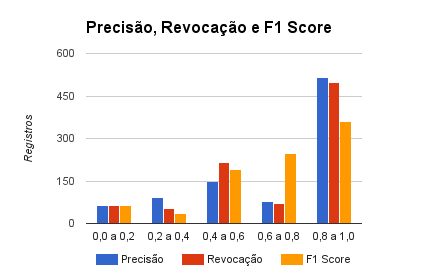
\includegraphics[scale=0.7]{medicoes}
	\caption{Distribuição das medições}
	\label{fig:medicoes}
\end{figure}


\section{Conclusão} \label{sec:conclusao}

[TODO]
\begin{itemize}
	\item Passar a definição formal do problema como segunda seção!
	\item Rodar cross-validation com todos os dados, atualizar a tabela e refazer os gráfico. É improvável um resultado muito diferente, então (espero) que eu não tenha que modificar o texto.
	\item Melhorar os gráficos. Achei que ficaram muito feios =/
	\item Observação: os resultados são intuitivamente muito bons mesmo quando a precisão não parece boa. Isso ainda precisa ser confirmado.
	\item Citar (UEDA; SAITO, 2002) com breve explicação. Propõem um método chamado Parametric Mixture Model para classificador binário.
	\item Explicar (DEMBCZYŃSKI et al., 2012) e (TAI; LIN, 2012) que também exploram as correlações entre rótulos para melhorar a classificação por Binary Relevance. Verificar também (ZHANG; ZHANG, 2010). Relacionar também com (ESULI; FAGNI; SEBASTIANI, 2008) que trabalha com hierarquia de rótulos, mas adaptando algoritmos
	\item Verificar se vale a pena citar (CHARTE et al., 2012) que propõe redução do número de rótulos através de regras de associação].
\end{itemize}

%%%%%%%%%%%%%%%%%%%%%%%%%%%%%%%%%%%%%%%%%%%%%%%%%%%%%%%%%%%%%%%%%%%%%%%%%%%%%%%
\bibliographystyle{splncs03}
\bibliography{paper}
%%%%%%%%%%%%%%%%%%%%%%%%%%%%%%%%%%%%%%%%%%%%%%%%%%%%%%%%%%%%%%%%%%%%%%%%%%%%%%%

\end{document}
